\begin{figure}[tb]
\centering
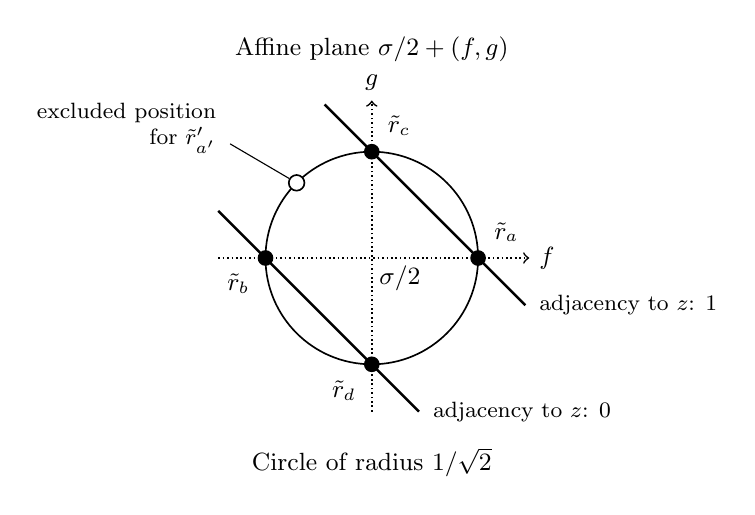
\begin{tikzpicture}[
  every node/.style={font=\small},
  point/.style={circle,fill=black,inner sep=2pt},
  candidate/.style={circle,draw,fill=white,inner sep=2pt},
  line width=.6pt,
]
\node at (0,2.65) {Affine plane $\sigma/2+\spn(f,g)$};
\draw[densely dotted,->] (-1.95,0)--(2,0) node[right] {$f$};
\draw[densely dotted,->] (0,-1.95)--(0,2) node[above] {$g$};
\draw (0,0) circle[radius=1.35];
\draw[line width=.9pt] (-.6,1.95)--(1.95,-.6);
\node[anchor=west,font=\footnotesize] at (2,-.6) {adjacency to $z$: $1$};
\draw[line width=.9pt] (-1.95,.6)--(.6,-1.95);
\node[anchor=west,font=\footnotesize] at (.65,-1.95) {adjacency to $z$: $0$};
\node[fill=white,inner sep=1pt,anchor=north west] at (.05,-.05) {$\sigma/2$};
\node[point,label=above right:$\tilde{r}_a$] at (1.35,0) {};
\node[point,label=below left:$\tilde{r}_b$] at (-1.35,0) {};
\node[point,label=above right:$\tilde{r}_c$] at (0,1.35) {};
\node[point,label=below left:$\tilde{r}_d$] at (0,-1.35) {};
\node[candidate] (excluded) at (135:1.35) {};
\node[anchor=east,align=right,font=\footnotesize] at (-1.85,1.65)
  {excluded position\\for $\tilde{r}'_{a'}$};
\draw[thin] (-1.8,1.45)--(excluded);
\node at (0,-2.6) {Circle of radius $1/\sqrt2$};
\end{tikzpicture}
\caption{Geometric interpretation of the calculation giving $\alpha\beta=0$.
The figure assumes that $z\in V(G)\setminus\supp u_0$ is adjacent to $a,c$
and not to $b,d$; the other cases of \cref{eq:quartet-probe} are symmetric.
For a candidate $\tilde{r}'_{a'}=\sigma/2+(\alpha f+\beta g)/\sqrt2$,
the circle gives $\alpha^2+\beta^2=1$.
By \cref{eq:integrality}, the two lines have equations
$\alpha+\beta=1$ and $\alpha+\beta=-1$.
Squaring either equation and subtracting the circle equation gives
$2\alpha\beta=0$. The hollow point is on the circle but off both lines,
so \cref{eq:integrality} excludes it.}
\label{fig:quartet-geometry}
\end{figure}
